\documentclass[a4paper,12pt]{article}
\usepackage[polish]{babel}
\usepackage[utf8]{inputenc}
\usepackage[T1]{fontenc}
\usepackage{times}
\usepackage{graphicx}
\usepackage{listings}
\usepackage[usenames,dvipsnames,svgnames]{xcolor}
\usepackage{geometry}
\usepackage{sidecap}
\usepackage{wrapfig}

\usepackage{amsfonts}
\usepackage{amsmath}

\usepackage{fancyhdr}

\pagestyle{fancy} %% deklarujemy styl "fancy"
\fancyhead{} \fancyfoot{} %% "zresetuj" zawartość pagin

\fancyhead[LE,RO]{\normalfont \small \thepage}
\fancyhead[LO]{\normalfont \small \itshape \rightmark}
\fancyhead[RE]{\normalfont \small \itshape \leftmark}
\fancypagestyle{plain}{\fancyhead{}\renewcommand{\headrulewidth}{0pt}} %% ustaw paginy dla stylu plain

\title{TITLE}
\author{AUTHOR}

\begin{document}

\maketitle

\section{Model HWIND}

Model łamliwości drzew HWIND powstał w celu wyznaczania maksymalnej prędkości wiatru przy których drzewo ulegnie złamaniu lub wyrwaniu (dla lasów sztucznie zalesianych). Został on opracowany dla sosny zwyczajnej i świerku pospolitego.

\begin{figure}[!h]
	\center
	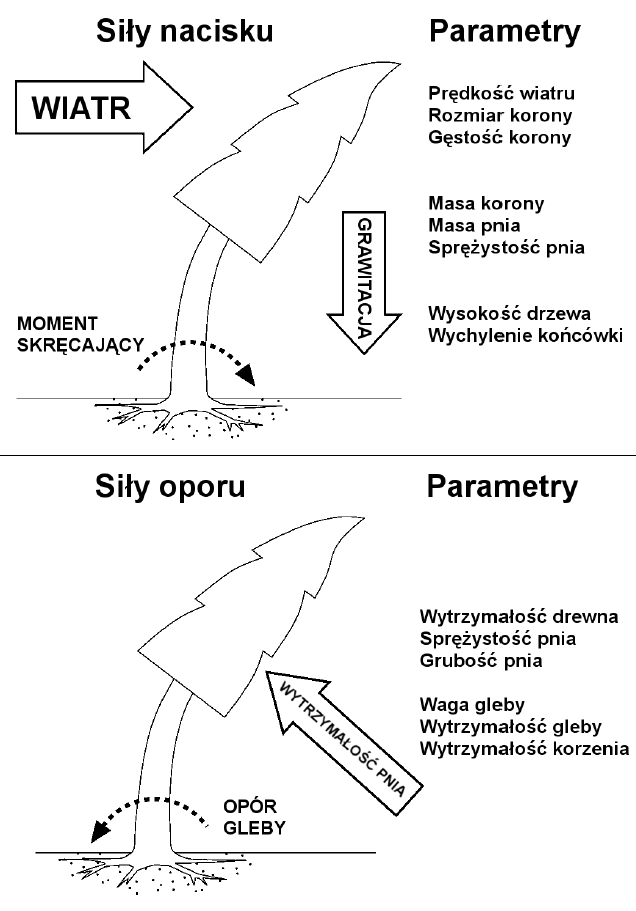
\includegraphics[scale=0.45]{HWIND1}
	\caption{Rozkład sił działających na drzewo dla modelu HWIND. Źródło: ~\cite{chm_mgza}.}
	\label{fig:HWIND1}
\end{figure} 

Rysunek ~\ref{fig:HWIND1} przedstawia siły działające na drzewo. Dokonany został podział na siły poziome i ~pionowe.
Pod naporem wiatru drzewo ugina się do momentu osiągnięcia punktu krytycznego, gdy siły nacisku (siła wiatru, siła grawitacji) zrównają się z ~siłami oporu (wytrzymałość pnia, wytrzymałość gleby wokół korzenia).

W celu wyznaczenia maksymalnego momentu skręcającego i ~granicznej prędkości wiatru przy której nastąpi zniszczenie drzewa, podzielone zostały one na 1~metrowe segmenty, dla których wyznaczone zostaną wartości sił.

Całkowita pozioma siła wiatru $F_w$ uzyskana zostaje poprzez sumowanie wartości siły wiatru obliczonej osobno dla każdego 1~metrowego segmentu ~\cite{chm_mgza}. Siła dla poszczególnego segmentu uzyskiwana jest ze wzoru:
$$ F_w(z) = \frac{1}{2}C_d  \rho v_h^2 A(z) $$ 
gdzie

\begin{description}
  \item[$C_d$] -- współczynnik tarcia
  \item[$\rho$ ]-- gęstość powietrza
  \item[$v_h$ ]-- prędkość pozioma dla danego segmentu
  \item[$A(z)$]-- przewidywana wielkość korony drzewa stawiająca opór wiatrowi
\end{description}

W celu uproszczenia obliczeń dokonana została aproksymacja powierzchni korony drzewa przez trójkąt równoramienny (świerk pospolity). Pole powierzchni pnia jest reprezentowane przez prostokąt. Model ten przedstawia rysunek \ref{fig:HWIND2}.

\begin{figure}[!h]
	\center
	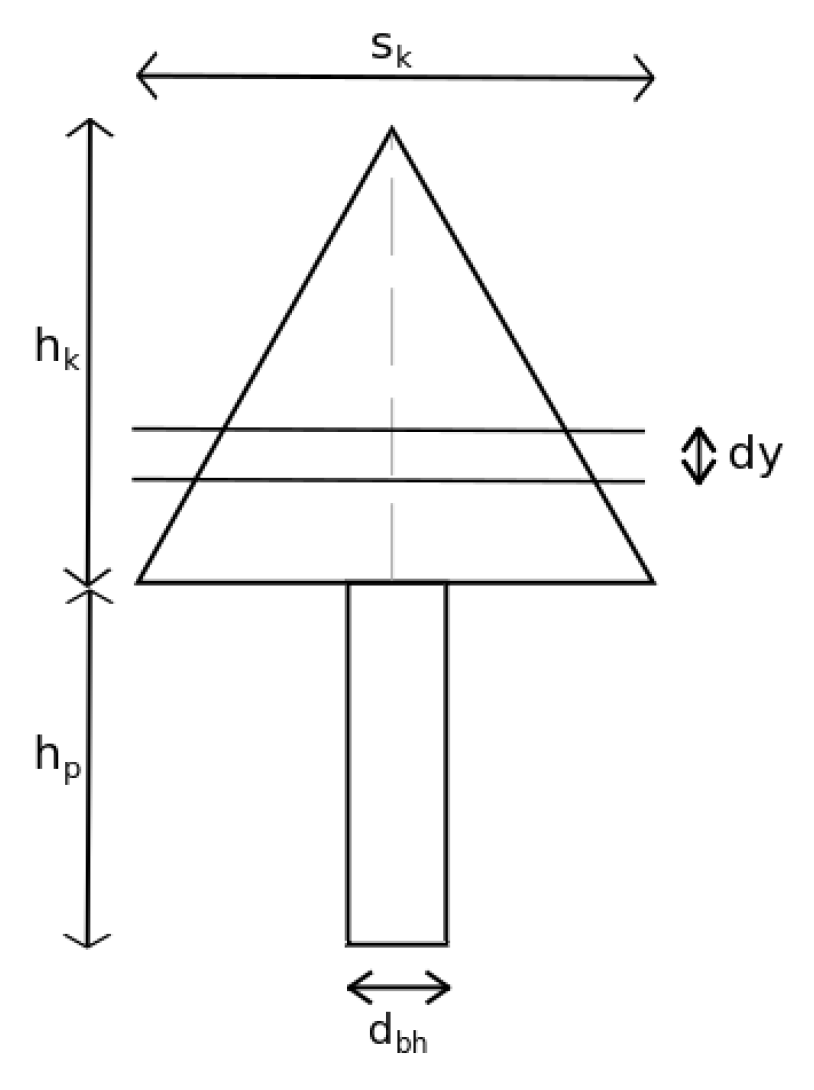
\includegraphics[scale=0.35]{HWIND2}
	\caption{Model powierzchni stawiającej opór wiatrowi. $s_k$ oznacza szerokość korony, $h_k$ -- wysokość korony, $h_p$ -- wysokość pnia, $d_{bh}$ -- średnicę pnia, $d_y$ -- wycinek powierzchni o wysokości 1m użyty przy w modelu HWIND. Źródło: ~\cite{chm_mgza}.}
	\label{fig:HWIND2}
\end{figure} 

W modelu należy uwzględnić fakt, iż pod wpływem wiatru powierzchnia korony ulega zmniejszeniu ~\cite{todo_jakies_zrodlo}. Redukcja powierzchni wynosi $20\%$ dla prędkości mniejszych od $11 \frac{m}{s}$, dla 
większych od $20\frac{m}{s}$ -- $60\%$. Dla wartości pomiędzy nimi współczynnik przepływu wiatru $S_t$ jest wyznaczany z następującego wzoru:
$$ S_t(z) = 0.044444v(z) - 0.28889$$
gdzie
\begin{description}
  \item[$v(z)$] -- prędkość wiatru na wysokości z
\end{description}

Powierzchnia $A(z)$ wyznaczana jest przez jej iloczyn ze współczynnikiem $S_t$.
\\

Siła grawitacji wyznaczana jest dla każdego segmentu drzewa, a następnie sumowana. Wyznaczana jest ze wzoru:
$$F_g(z) = m_c g$$
gdzie
\begin{description}
  \item[$m_c$] -- masa korony drzewa
  \item[$g$] -- przyspieszenie ziemskie
\end{description}

\input{Rankine}


\bibliography{books}{}
\bibliographystyle{plain}
\end{document}




